\section{Design}
\subsection{Block Diagrams}
The design of this project is modular in nature. It is desired to have one main controller and
multiple remote temperature sensors and vent controllers, as shown in Fig.~\ref{fig:maindiagram}. Fig.~\ref{fig:cntldiagram} will show the main control panel in more detail, while Fig.~\ref{fig:remotediagram} will show the remote temperature sensors, and Fig.~\ref{fig:remotediagram} will show the vent controllers.  Each component will be described in further detail in \S\ref{sect:blockdescriptions}.

\begin{figure}[htb]
\centering
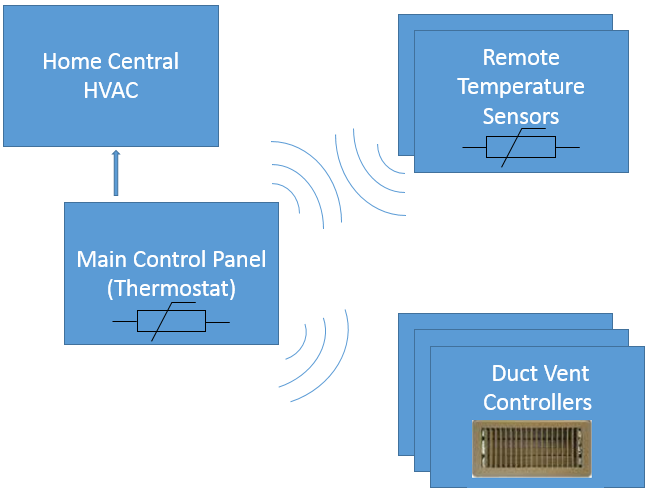
\includegraphics[width=.9\textwidth]{OverallDiagram.png}
\caption{Top level system diagram.}
\label{fig:maindiagram}
\end{figure}

\begin{figure}[htb]
\centering
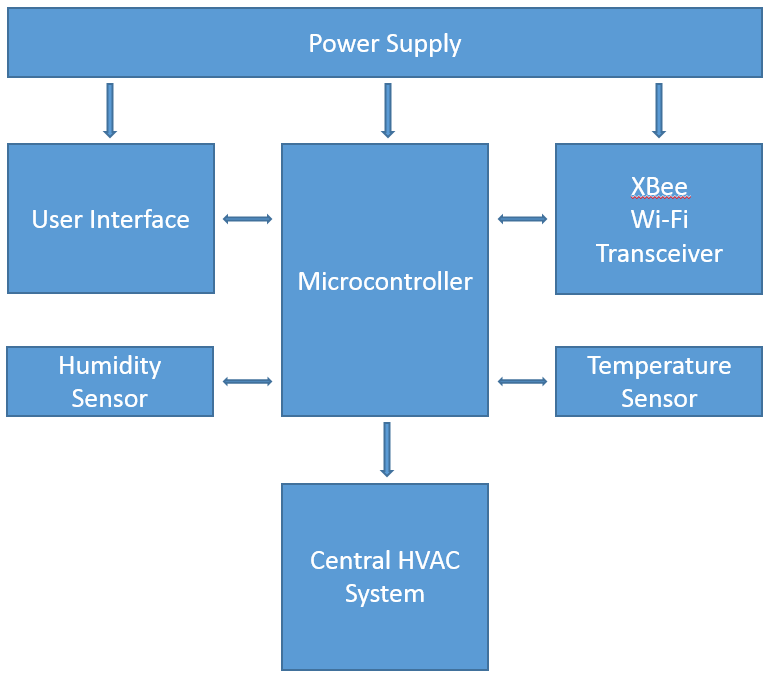
\includegraphics[width=.9\textwidth]{MainCntlBlockDiagram.png}
\caption{Main Control Panel component Diagram from Fig.~\ref{fig:maindiagram}.}
\label{fig:cntldiagram}
\end{figure}

\begin{figure}[htb]
\centering
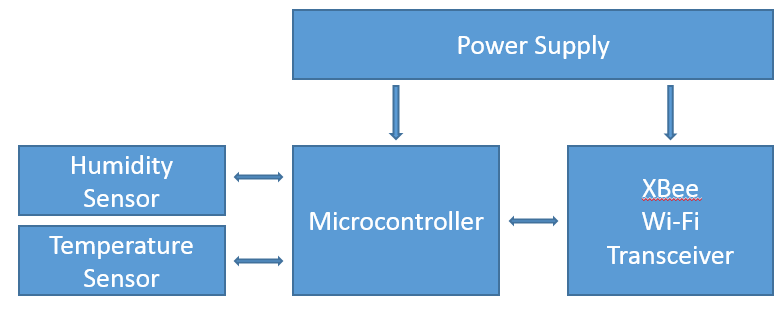
\includegraphics[width=.9\textwidth]{RemotePanelDiagram.png}
\caption{Remote Temperature Sensor component diagram from Fig.~\ref{fig:maindiagram}.}
\label{fig:remotediagram}
\end{figure}

\begin{figure}[htb]
\centering
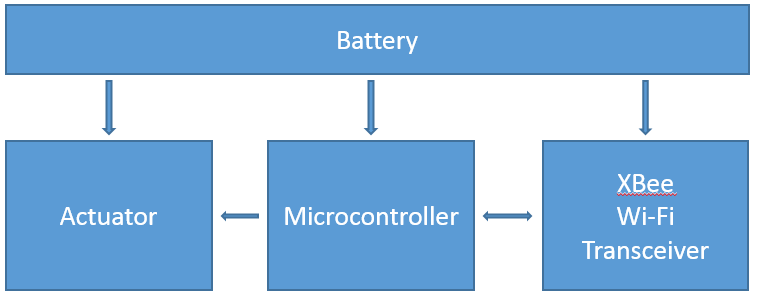
\includegraphics[width=.9\textwidth]{VentCntlDiagram.png}
\caption{Vent Duct Controller component diagram from Fig.~\ref{fig:maindiagram}.}
\label{fig:ventdiagram}
\end{figure}

\subsection{Block Descriptions}
\label{sect:blockdescriptions}
\subsubsection{Overall System Summary}
The overall system will consist of one main control panel, a central HVAC system, and any number of remote temperature sensors and duct vent controllers.  At least one remote temperature sensor is required for the system to be ``smart'', such that it will be able to detect temperatures in rooms other than where the normal thermostat (main control panel) is located.  The duct vent controllers also follow a similar logic, as many duct controllers would be used as desired to control air flow to desired rooms, but at least two are required to make the system work as intended.
%There are several components used in many of the components: temperature and humidity sensors, microcontrollers, and wireless transceivers.
\paragraph{Temperature Sensors}
\label{Temp Sensors}
An LM35 temperature sensor is used to get an accurate reading of temperature in all components. The sensors will be read by the microcontrollers and used along with humidity sensors to determine HVAC on/off state and vents open/closed state.
\paragraph{Humidity Sensors}
\label{humid_sensors}
An HH10D humidity sensor will be used to measure the relative humidity around the sensor.  The humidity reading will be used along with the temperature reading to set the temperatures in each room.

\paragraph{Central HVAC}
No modifications to a home's central HVAC system was desired. In the United States, most central HVAC systems use a 5-wire system as seen in Fig.~\ref{fig:5wire}.  The 5 wire system consists of a $24VAC$ red supply wire with blue/cyan neutral.  The white, yellow, and green wires correspond to relays which are turned on by 24VAC supplied to them. It is the job of the thermostat to switch the 24VAC power to each of the desired system relays.  Light bulbs were connected to the main panel's green,white, and yellow wires to verify that the main panel would properly turn on and off the HVAC system.  The main panel was also designed to utilize this 24VAC source.

\begin{figure}
\centering
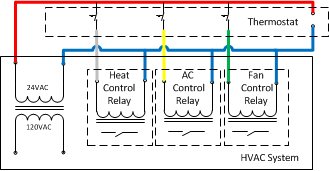
\includegraphics[width=.99\textwidth]{5wire.png}
\caption{Basic schematic for a 5-wire HVAC system found in many homes.}
\label{fig:5wire}
\end{figure}

%Begin Main Panel Design Section
\subsubsection{Main Control Panel}
The main control panel acts as master to all other components. The main control panel can be broken down into several components as shown in Fig.~\ref{fig:cntldiagram}. Fig.~\ref{fig:main_cntl_schematic} gives a closer look at the main control panel.  The main control panel was broken into smaller parts for verification reasons: HVAC system, Power Supply, Microcontroller, and XBee Wi-Fi.

The main control panel was housed in a prototype box from RadioShack.  The enclosure hid much of the wires, protecting the user from the open wires, and was more aesthetically pleasing. Fig.~\ref{fig:main_panel_box} shows the completed main control panel during operation.  Fig.~\ref{fig:main_panel_apart}
\begin{figure}
\centering
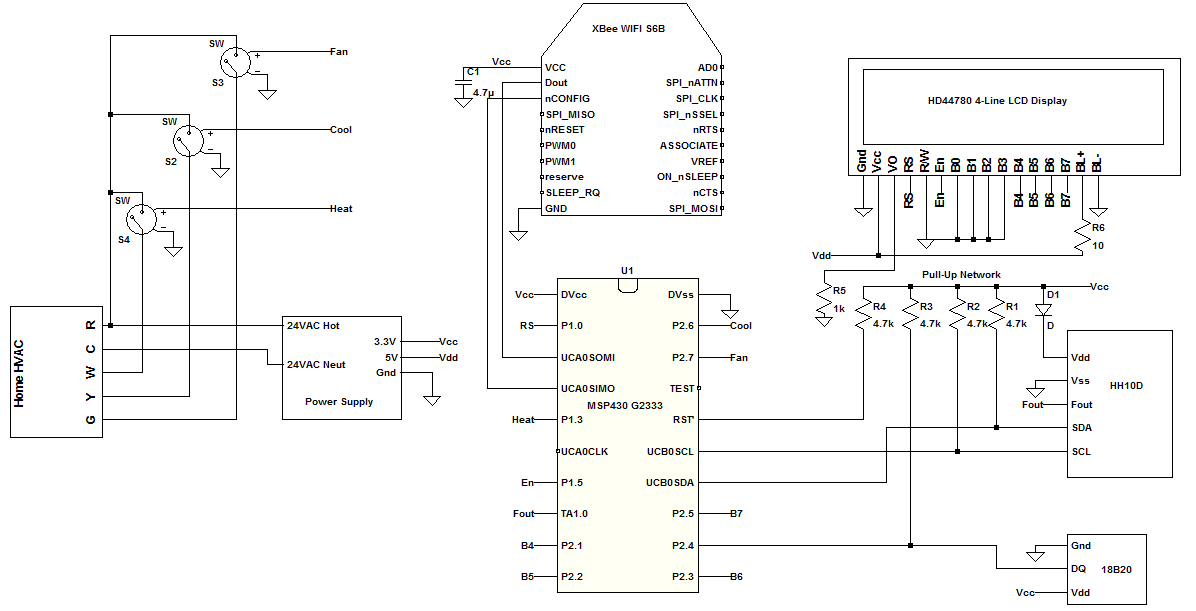
\includegraphics[width=.99\textwidth]{main_cntl_schematic.png}
\caption{Main control panel schematic.}
\label{fig:main_cntl_schematic}
\end{figure}

\begin{figure}
\centering
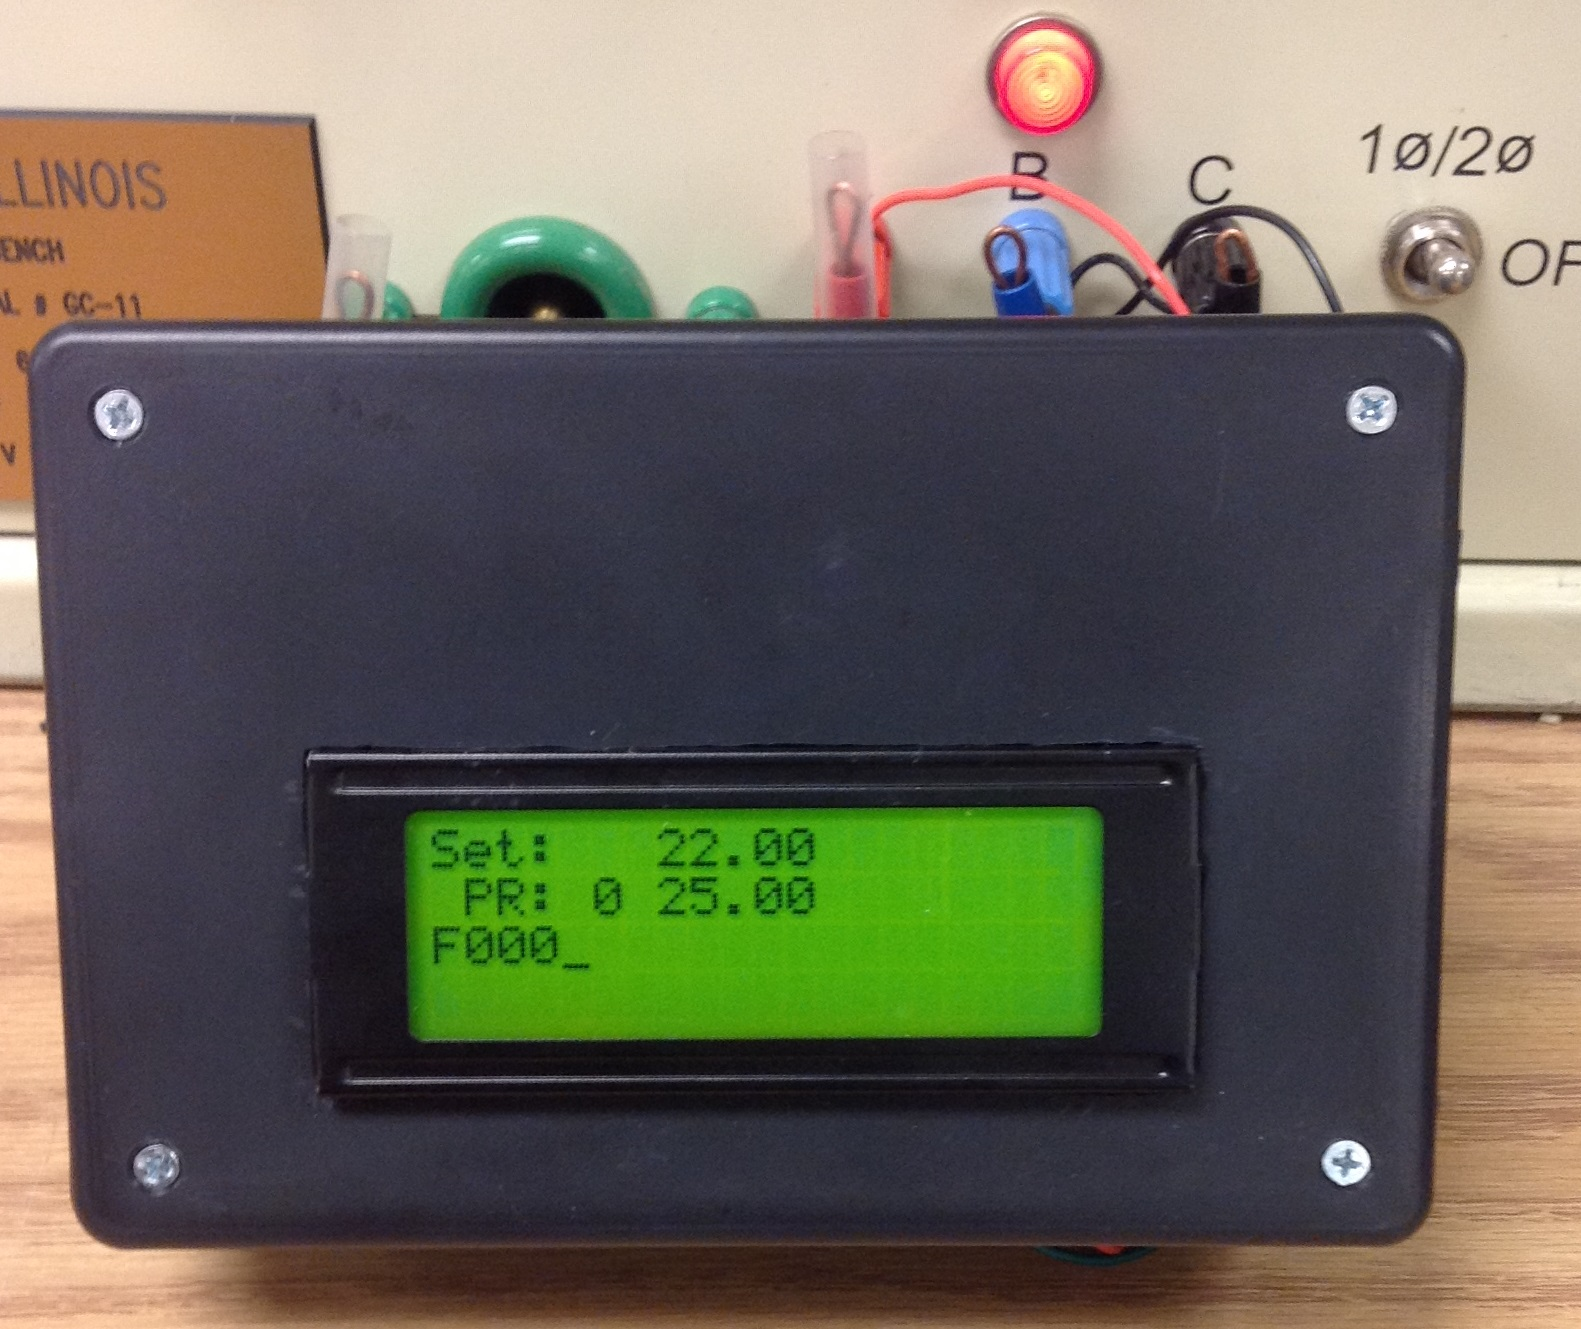
\includegraphics[width=.99\textwidth]{main_panel_box.png}
\caption{Main control panel inside its enclosure, operating.}
\label{fig:main_panel_box}
\end{figure}

\begin{figure}
\centering
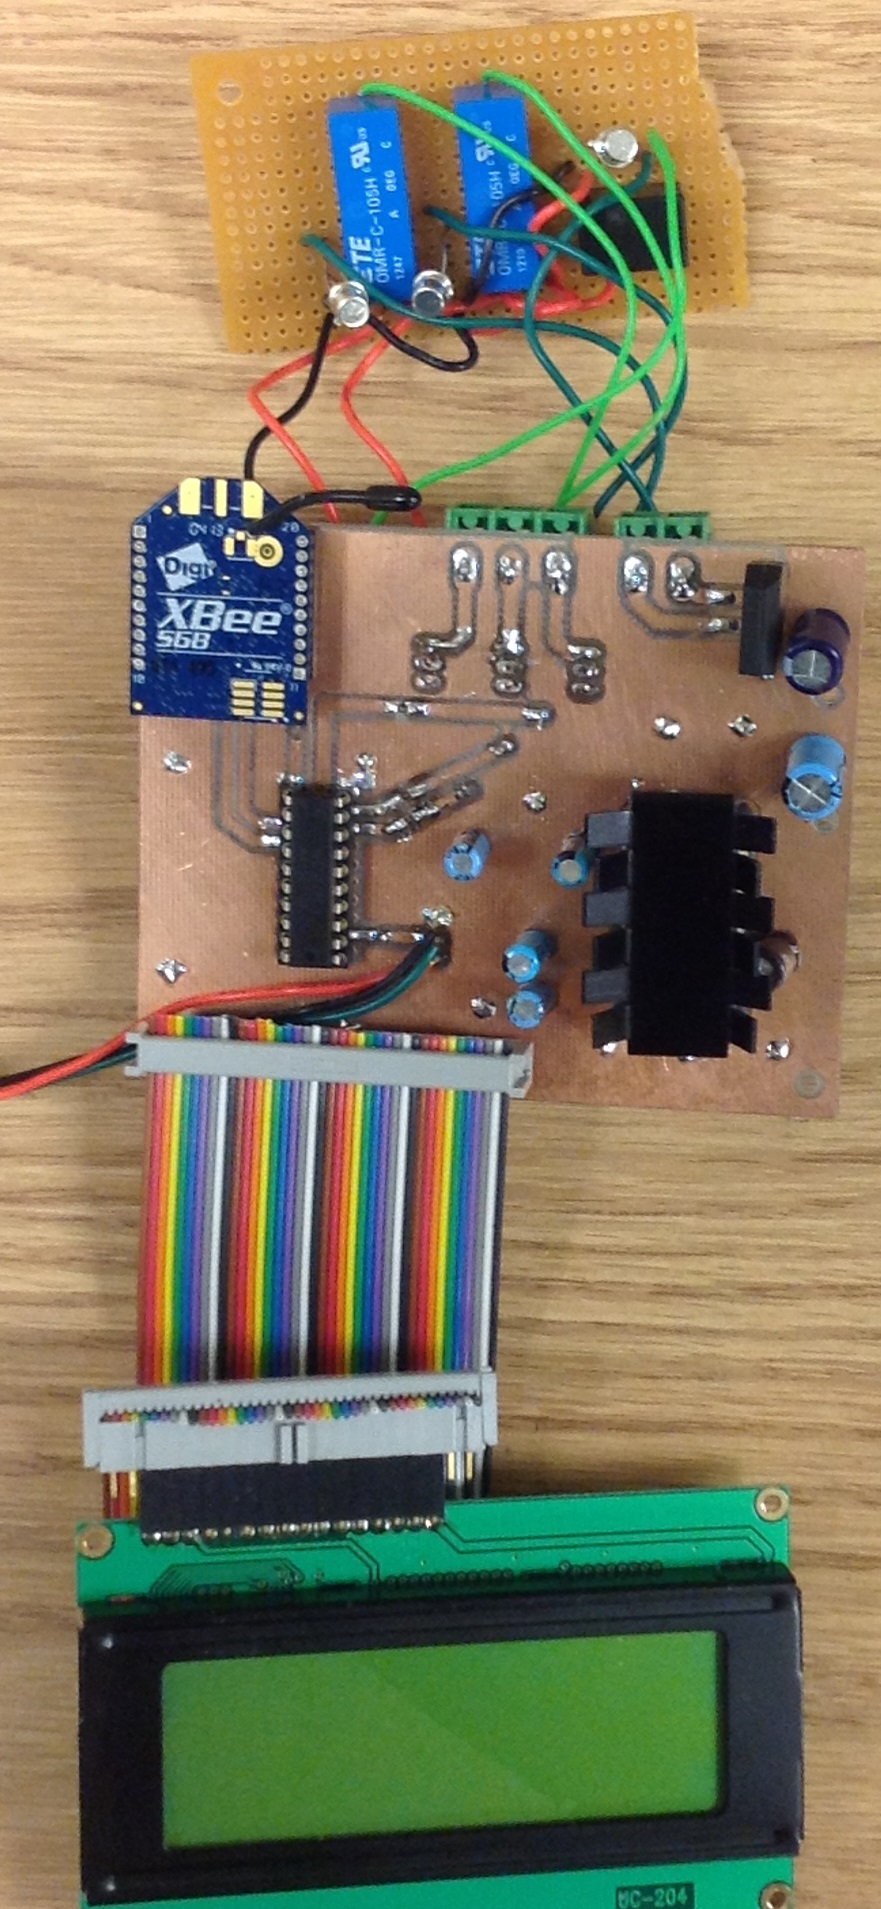
\includegraphics[width=.99\textwidth]{main_panel_apart.png}
\caption{Disassembled main control panel, showing main board, relay board, and LCD.}
\label{fig:main_panel_apart}
\end{figure}

\paragraph{Main Panel Power Supply}
The Main Control Panel is to be powered by the 24VAC low-voltage supply from a home's HVAC system. The 24VAC was rectified using a NTE167 bridge rectifier in KBPM package.  Filtering capacitors provided a more constant input, Fig.~\ref{fig:main_rectified}, to an integrated power supply from TI, the LM2825-5.0.  The LM2825-5.0 is a buck converter integrated into a $.6"$ DIP24 package, and provides a constant 5V output with very little loss at up to 1A.  This 5V was appropriate for powering the UC204 LCD (Hitachi HD44780 protocol; see the User Interface section) and an LT1129-3.3 LDO regulator, from Linear Technology, capable of supplying the $3.3VDC$ necessary for the XBee and UC-204A LCD (Hitachi HD44780; User Interface section). Figures~\ref{fig:main_5v_output} and~\ref{fig:main_3_3v_output} display the verified operation of the power supplies.

This power supply design differs from the proposed design in several ways.  The LM2825-5.0 was a late design change and replaced the original DC-DC converter design.  This is due to unforeseen issues with the original converter.  Because the converter design was not critical or the focus of the project, the LM2825-5.0 was worked into the design as a replacement during a PCB rework.  This substitution saved a great deal of troubleshooting time and allowed the project to be completed on time, but changed proposed cost slightly.

\begin{figure}
\centering
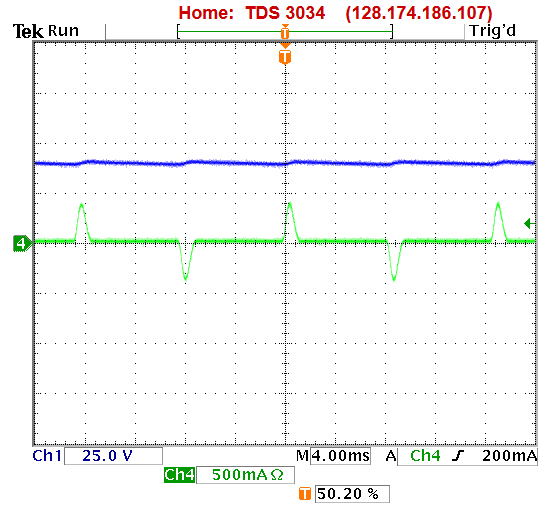
\includegraphics[width=.99\textwidth]{main_rectified_input.png}
\caption{Rectified and filtered 24VAC input to the main panel.}
\label{fig:main_rectified}
\end{figure}
\begin{figure}
\centering
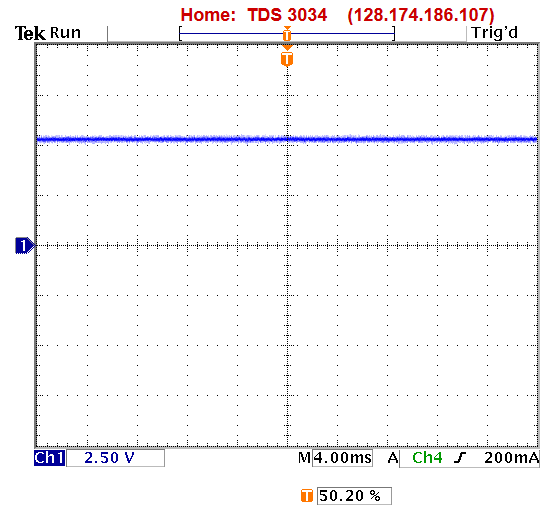
\includegraphics[width=.8\textwidth]{main_5v_output.png}
\caption{5V output measurement from the LM2825-5.0 integrated power converter.}
\label{fig:main_5v_output}
\end{figure}
\begin{figure}
\centering
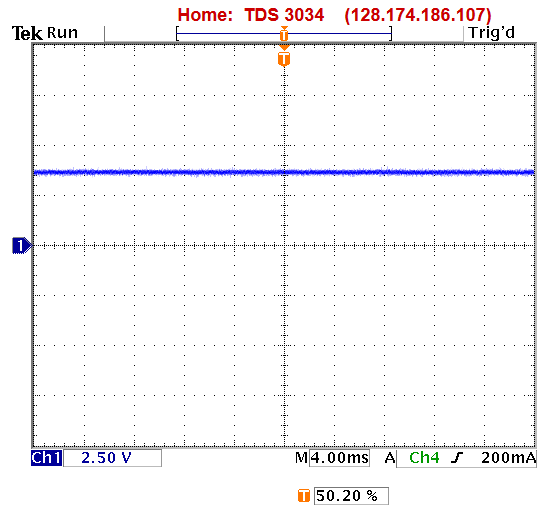
\includegraphics[width=.8\textwidth]{main_3_3v_output.png}
\caption{3.3V output measurement from the LT1129-3.3 LDO regulator.}
\label{fig:main_3_3v_output}
\end{figure}

\paragraph{Main Panel Microcontroller}
\begin{figure}
\centering
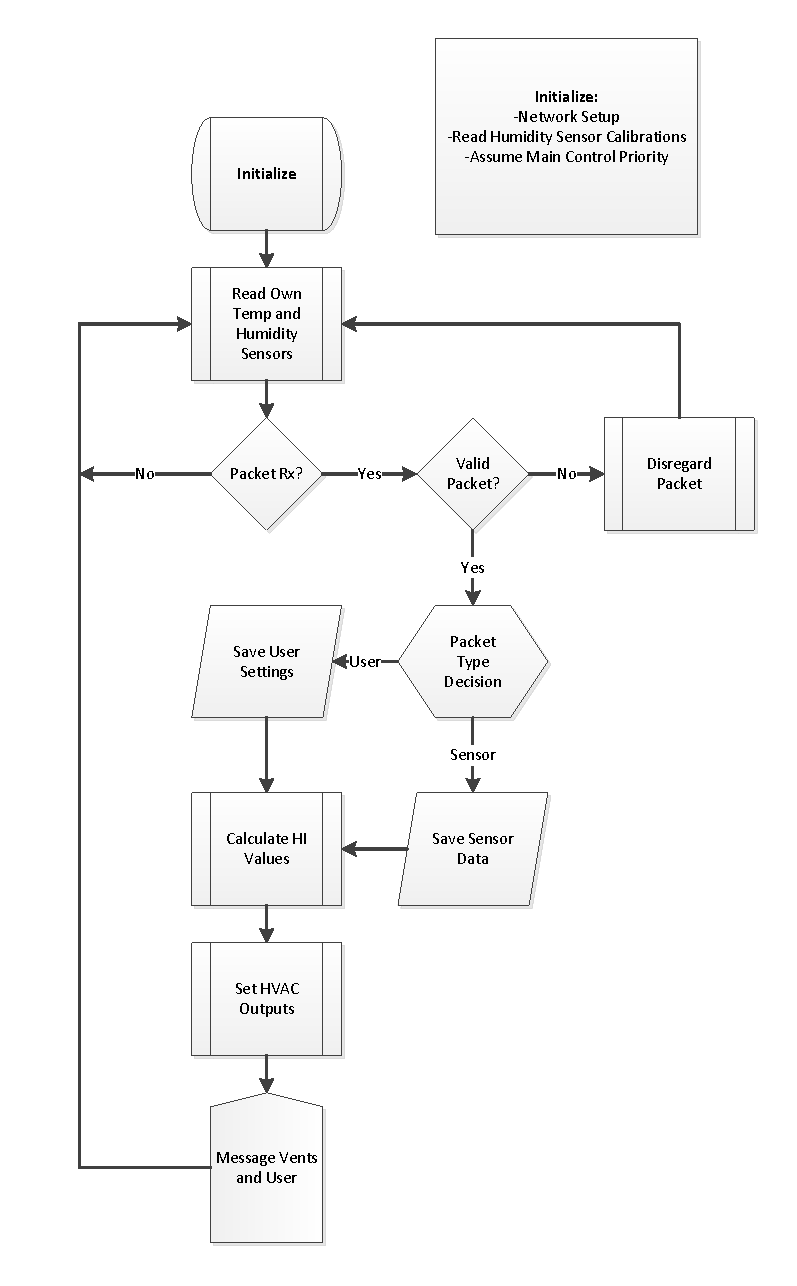
\includegraphics[height=.9\textheight]{maincntl_flow.pdf}
\caption{Flow chart depicting MSP430 programmed control logic.}
\label{fig:maincntl_flow}
\end{figure}

The microcontroller used will be an MSP430 microcontroller. The microcontroller must send and receive packets over the network via the wireless transceiver, read the temperature and humidity sensors, signal the central HVAC system on or off, and output to an LCD display for debugging and UI purposes. The main control panel will receive broadcast data from all of the remote temperature sensors on the network (including its own sensors). Once the microcontroller receives temperature information from each remote sensor, it determines which vents to open and close and sends data wirelessly to the desired vent controllers. The HVAC is controlled over a 2-3 wire system connected directly to the HVAC over existing house wiring.
% Table generated by Excel2LaTeX from sheet 'Sheet1'
\begin{table}[htbp]
\centering
\caption{MSP430G2333 Designed Pin Assignments.}
\begin{tabular}{|c|c|c|}
\hline
\textbf{\#} & \textbf{MSP430 Pin} & \textbf{Function} \bigstrut\\
\hline
\hline
1 & DVcc & 3.3V power input \bigstrut\\
\hline
2 & P1.0 & LCD Register Select \bigstrut\\
\hline
3 & UCA0 Rxd & XBee Dout \bigstrut\\
\hline
4 & UCA0 Txd & XBee Din \bigstrut\\
\hline
5 & P1.3 & HVAC Heat ON switch \bigstrut\\
\hline
6 & N/C \bigstrut\\
\hline
7 & P1.5 & LCD Enable \bigstrut\\
\hline
8 & TA1.0 & Temp Sensor Fout \bigstrut\\
\hline
9 & P2.1 & LCD Bit 0 \bigstrut\\
\hline
10 & P2.2 & LCD Bit 1 \bigstrut\\
\hline
11 & DVss & Gnd \bigstrut\\
\hline
12 & P2.6 & HVAC Cool ON switch \bigstrut\\
\hline
13 & P2.7 & HVAC Fan ON switch \bigstrut\\
\hline
14 & TEST & N/C \bigstrut\\
\hline
15 & RST & 3.3V tied high \bigstrut\\
\hline
16 & UCB0SCL & Temp Sensor SCL \bigstrut\\
\hline
17 & UCB0SDA & Temp Sensor SDA \bigstrut\\
\hline
18 & P2.5 & LCD Bit 2 \bigstrut\\
\hline
19 & P2.4 & Humidity Sensor DQ \bigstrut\\
\hline
20 & P2.3 & LCD Bit 3 \bigstrut\\
\hline
\end{tabular}%
\label{tab:msp_inout}%
\end{table}%

\paragraph{XBee Wi-Fi Transceiver}
The Xbee transciever block is the main communication portion of the design. The transceivers will all be on a wireless network to allow each component to send/receive messages from the main control panel. Power for the transceiver is $3.3\vdc$ and comes from the power supply. The transceiver connects to the microcontroller via serial port.

\paragraph{Main Panel Temperature and Humidity Sensors}
See \S\ref{temp_sensors} and \S\ref{humid_sensors}.

\paragraph{Main Panel User Interface}
Interfacing with the main control panel was done in two parts. An HD44780 Hitachi LCD display was used to display current system settings and temperature at the main panel. To program the thermostat, a user interface application was written in C\# in Visual Studio 2010. Users can change room priorities, temperature preferences, and whether the system is in A/C mode or Heat. 

The PC application follows the flow chart in Fig.~\ref{fig:PCapp_flow}. Fig.~\ref{fig:PC_app} shows the PC application GUI, which has been tested on Windows machines only.  To communicate with the main panel, the PC must be connected to the same local network.  The PC app assembles a 10 byte message, including a unique header, which is sent to the main panel.  The message format can be seen in Fig.~\ref{fig:pcapp_message}.

\begin{figure}
\centering
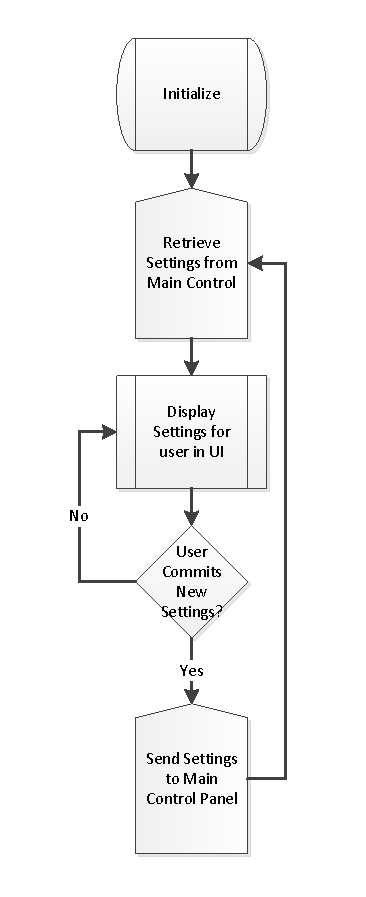
\includegraphics[width=.4\textwidth]{PCapp_flow.pdf}
\caption{Flow chart depicting the PC application logic flow.}
\label{fig:PCapp_flow}
\end{figure}


\begin{figure}
\centering
\includegraphics[width=.9\textwidth]{PC_app.png}
\caption{Screen shot of the PC App GUI.}
\label{fig:PC_app}
\end{figure}

\begin{figure}
\centering
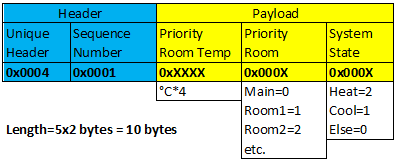
\includegraphics[width=.9\textwidth]{pcapp_message.png}
\caption{PC app control message sent to the main panel on user command.}
\label{fig:pcapp_message}
\end{figure}

The HD44780 protocol display was realized through a UC-204A type LCD.  This LCD has built a built in backlight and is capable of displaying 4 rows of 20 characters.  It requires 5VDC to supply both the logic circuitry and the backlight (current controlled); however the logic was drivable with 3.3VDC from the MSP430 and powered with 5VDC. Fig.~\ref{fig:lcd_sample} shows the LCD with some currently displayed items.

\begin{figure}
\centering
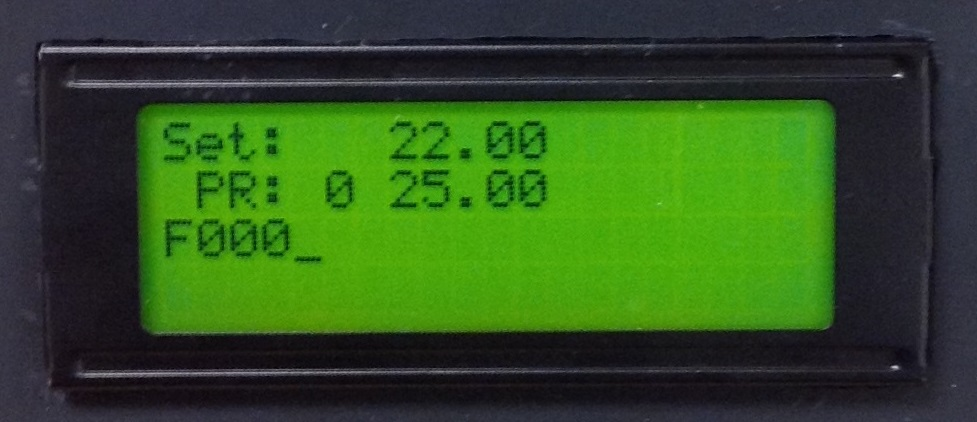
\includegraphics[width=.9\textwidth]{LCD_sample.png}
\caption{UC-204A LCD displaying temperature information.  The top line is the commanded temperature in $^\circ C$, followed by the current priority room temperature.  Priority room is displayed in numeric format (the same number as was sent by the PC App).  The 3rd line is debugging information which correlates to the Wi-Fi connections of the other system components. }
\label{fig:lcd_sample}
\end{figure}

%end main control panel design



%Begin Remote Temperature Sensor Design
\begin{figure} [htb]
\centering
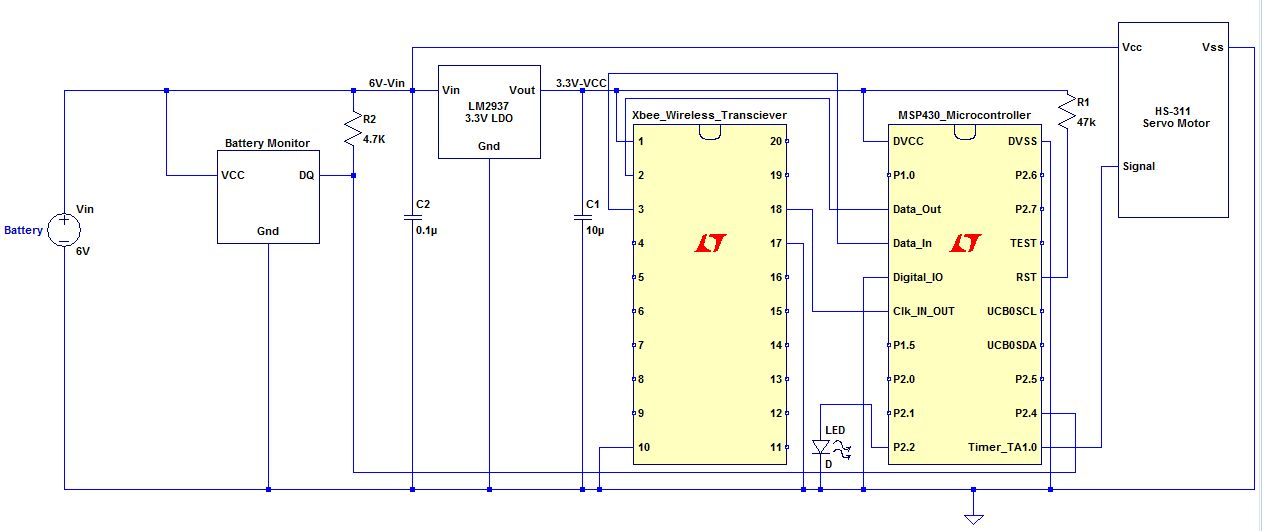
\includegraphics[width=.99\textwidth]{Temperature_Sensor.JPG}
\caption{Temperature Control System schematic.}
\label{fig:Temperature_System}
\end{figure}


\subsubsection{Remote Temperature Sensors}
A remote temperature sensor consists of a power supply, microcontroller, sensors, and wireless transceiver as shown in Fig.~\ref{fig:remotediagram}.  Each remote temperature sensor will be identical, and will be housed in a small plastic case and plugged into an AC outlet.
\paragraph{Remote Temperature Sensor Power Supply}
The power source for this component is a standard AC outlet.  Like the main controller, an AC-DC converter is required to convert the 120\,VAC\,(RMS) into the 3.3\,VDC required by the microcontroller and wireless transceiver.  The conversion will be done using a standard ``USB style'' power supply.
\paragraph{Remote Temperature Sensor Microcontroller}
The MCU is a TI MSP430G2333.  It will read the temperature and humidity sensors and periodically send the data to the main controller via a Wifi network connection.  The MCU is responsible for initializing the XBee with the appropriate network configuration parameters, and reading the proper calibration parameters from the humidity sensor via the I$^2$C bus.
\paragraph{Remote Temperature Sensor XBee Transceiver}
The Xbee transceiver is used in the remote sensor to allow communication to the main control panel. It will be interfaced to the microcontroller via SPI port.  The Xbee will connect to a pre-determined network.
%End Design

%Begin Vent Controller Design
\begin{figure} [htb]
\centering
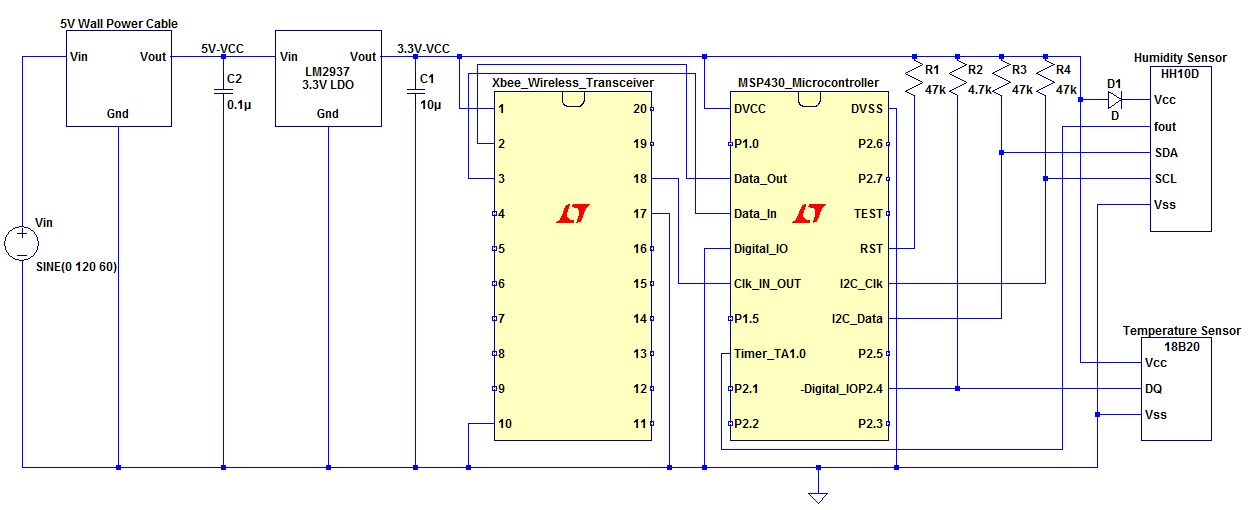
\includegraphics[width=.99\textwidth]{Vent_System.JPG}
\caption{Vent Control System schematic.}
\label{fig:Vent_System}
\end{figure}

\subsubsection{Vent Controllers}
The vent controller, shown in Fig.~\ref{fig:ventdiagram}, will mount inside of a standard HVAC ventilation cover and control the opening and closing of the vent.  Opening and closing of the vent will allow the system control over HVAC flow out of the desired vent, and by extension, the room. The vent controller will receive messages from the main control panel and open or close the vent using an actuator connected to the vent's existing closer. Each vent controller will be identical and can be replicated as desired.
\paragraph{Vent Controller Battery}
Since many homes have vents which are not near AC outlets, and it is not desirable to add a great deal of house wiring, the vent controllers will be battery powered.  4 AA batteries will be used to supply power to the microcontroller, transceiver, and actuator motor.
\paragraph{Battery Monitor}
\paragraph{Vent Controller Microcontroller}
The MSP430 is used to receive messages from the main control panel via the wireless transceiver.  The MCU is responsible for initializing the XBee with the correct network configuration parameters.  Once the appropriate packet is received, the controller will command a DC actuator to open/close the vent.
\paragraph{Vent Controller XBee Transceiver}
The wireless transceiver in the vent controller will receive only. It will receive messages via the wireless network and forward the message via an SPI connection.
\paragraph{Vent Controller Actuator}
We will be using the HS-311 Servo motor controlled by a MSP430 microcontroller and will be powered by 4 AA batteries to ensure a 6V output. The motors position will be controlled by a square wave sent from the MCU. The neutral position pulse duration is 1.5\,ms, which corresponds to 90$^{\circ}$ and any pulse width below that drives the servo toward 0$^{\circ}$, while a pulse longer than 1.5\,ms drives it toward 180$^{\circ}$. The ``Vent off'' position will be at 180$^{\circ}$ and ``Vent on'' position will be at 90$^{\circ}$.
%end design
